% Project Proposal Document
\documentclass[final]{cmpreport}
\makeatletter
\input{t1pcr.fd}
\makeatother
\setlength{\footnotesep}{3ex}
\title{\Codex: A Progressive Web App in React for table-top role-playing games}
\author{Christopher Alastair Irvine}
\registration{100036248}
\supervisor{Dr Katharina Huber}
\ccode{CMP-6013Y}
\summary{This project is the tits and here's why...}
\acknowledgements{
	I would like to thank Dr Katharina Huber for taking on the supervision of this project, 
	and guiding me towards success. Additionally I would like to thank Wizards of the Coast 
	for their generosity and kindness in allowing the use of their Intellectual Property for this project.
}
\usepackage{rotating}
\usepackage{csquotes}
\usepackage{hhline}
\usepackage{caption}
\usepackage{makecell}
\usepackage{listings}
\newcommand{\ueacmp}{UEA School of Computing Sciences}
\newcommand{\WotC}{Wizards of the Coast}
\newcommand{\dnd}{D\&D}
\newcommand{\sem}{Software Engineering Model}
\newcommand{\sems}{Software Engineering Models}
\newcommand{\Codex}{\textsc{Codex}}
\newcommand{\AgileSolo}{\emph{Agile Solo}}
\graphicspath{ {Images/} }
\lstdefinelanguage{JavaScript}{
	keywords={typeof, new, true, false, catch, function, return, null, catch, switch, var, if, in, while, do, else, case, break},
	keywordstyle=\color{blue}\bfseries,
	ndkeywords={class, export, boolean, throw, implements, import, this},
	ndkeywordstyle=\color{darkgray}\bfseries,
	identifierstyle=\color{black},
	sensitive=false,
	comment=[l]{//},
	morecomment=[s]{/*}{*/},
	commentstyle=\color{purple}\ttfamily,
	stringstyle=\color{red}\ttfamily,
	morestring=[b]',
	morestring=[b]"
}
\lstset{
	language=JavaScript,
	backgroundcolor=\color{lightgray},
	extendedchars=true,
	basicstyle=\footnotesize\ttfamily,
	showstringspaces=false,
	showspaces=false,
	numbers=left,
	numberstyle=\footnotesize,
	numbersep=9pt,
	tabsize=2,
	breaklines=true,
	showtabs=false,
	captionpos=b
}
% EOF Preamble and Macros
	
% BOF Document
\begin{document}	
	% BOF Introduction
	\section{Introduction} \label{sec:introduction}
	hello there
	\begin{cmpfigure}{\Codex \ Gantt Chart, outlining the major tasks and deliverables\label{gantt:pplan}}
		\begin{sideways}
			\newganttchartelement{voidbar}{
				voidbar/.style={draw=black, top color=black!25, bottom color=black!23
			}}
			\begin{ganttchart}[y unit chart = 0.75cm, y unit title = 0.75cm, x unit=0.45cm, vgrid, title label font=\scriptsize,
				canvas/.style={draw=black, dotted}]{1}{34}
				\gantttitle{Project schedule shown for e-vision week numbers
					and semester week numbers}{34} \\
				
				\gantttitlelist{8,...,41}{1}\\
				\gantttitlelist{1,...,12}{1} \gantttitle{CB}{4}
				\gantttitlelist{1,...,9}{1} \gantttitle{EB}{4}
				\gantttitlelist{10,...,14}{1}\\
				
				%The elements, bars and milestones, are identified as elem0, elem1, etc.
				\ganttbar{Project Proposal}{1}{2} \\        		%elem0  
				\ganttbar{Literature Review}{2}{5} \\      			%elem1 
				\ganttmilestone{Literature Review Finished}{5} \\	%elem2
				\ganttbar{Design 1}{4}{8} \\ 						%elem3
				\ganttbar{Development 1}{9}{11} \\					%elem4
				\ganttbar{Progress Report}{11}{12} 					%elem5
				\ganttmilestone{}{12} \\							%elem6
				\ganttbar{Development 2}{11}{12}  		 			%elem7
				%week 1 of semester 2 is the 17th week in schedule 
				\ganttvoidbar{}{13}{16} \\                     		%elem8
				\ganttbar{Report Writing 1}{17}{19} 	        	%elem9
				\ganttmilestone{}{19} \\							%elem10
				\ganttbar{Design 2}{19}{20} \\      				%elem11
				\ganttbar{Development 3}{21}{26} \\					%elem12
				\ganttbar{Testing}{24}{26} \\						%elem13
				\ganttmilestone{Code Delivery}{26} \\       		%elem14
				\ganttbar{Report Writing 2}{27}{30} \\  			%elem15
				\ganttbar{Demonstration preparation}{31}{34}   		%elem16
				
				\ganttlink{elem0}{elem1} \ganttlink{elem1}{elem2} \ganttlink{elem2}{elem3}
				\ganttlink{elem3}{elem4} \ganttlink{elem4}{elem5} \ganttlink{elem5}{elem6}
				\ganttlink{elem5}{elem7} \ganttlink{elem8}{elem9} \ganttlink{elem10}{elem11}
				\ganttlink{elem11}{elem12} \ganttlink{elem12}{elem13} 
				\ganttlink{elem13}{elem14} \ganttlink{elem14}{elem15}
				\ganttlink{elem15}{elem16}
			\end{ganttchart}
		\end{sideways}
	\end{cmpfigure}		
	\section{What is \Codex?} \label{sec:what-codex}
	\Codex \ was a project that has two components. The first, produce a progressive web app built in ReactJS that was developed using a single developer Agile software engineering methodology, the second component was to evaluate the quality of that methodology. By the end of this section we will have an appreciation of the \Codex \ app, in terms of both context and purpose (see Sections \ref{sec:context}).
	
		\subsection{Context} \label{sec:context}
		The \Codex \ an app was based around the popular tabletop role-playing game known as Dungeons and Dragons (\dnd), created and published by \WotC. This game, and the principles that bring the game to life, drove the requirements which formed the basic structure of the \Codex \ app. Therefore, in order to understand the functionality, principle and importance of the \Codex \ app, we must first gain an understanding of \dnd. 
		
		The author of this paper has multiple years of experience with \dnd, both as a \emph{Player} and \emph{Dungeon Master} (DM). The \Codex \ app began as a personal project for the author of this paper, which grew into a tool to evaluate a single developer Agile software engineering methodology. 
		
			\subsubsection{What is Dungeons and Dragons?} \label{sec:what-dnd}
			The game of \dnd, at time of writing, was a popular tabletop role-playing game where a group of friends engage in a grand fantasy adventure powered by a narrative (\cite{DnDOriginal}, \cite{DnDHistory}). The story would be divided into manageable blocks of time known as \emph{sessions}. Each session may take between two and four hours to run, however this is not strictly enforced and is decided by the group of players. The events of each session, and the larger campaign, was created and controlled by a player known as the \emph{Dungeon Master} (DM) (for more details on DMs please see Section \ref{sec:dm-vs-player}). However, the campaign would not always occur as written. The players, who were clueless as to the next plot in the campaign, might take the story in an entirely different direction several times a session. The DM would have to react to these unexpected inputs and redraw the narrative during each session, or attempt to guide the players subtly back on track \citep{PlayerHandbook}. 
			
			Whilst it was possible for DMs to purchase pre-written campaigns, published either by experienced DMs or \WotC, many DMs would take it upon themselves to create their own worlds in which the campaign would occur or alter the pre-written campaigns to suit the needs of the group. For every game of \dnd \ was inherently different from each other, including those following the same campaign book. Because of this difference it was hard to estimate how many sessions a campaign might take. 
			
			The players would form an entity known as the \emph{party}, that would consist of the characters that the players embodied for the duration of the campaign. Each player controls one character, known as the \emph{player character}, within the party. The party would serve as the groups device in how they interact with the world, this is true for the DM who would not embody one character, but every other character within the world. These characters would be referred to ask \emph{non-player characters} and would include both allies and enemies of the party. For that reason, the external perception of the \dnd \ might be that the players were against the DM. Nothing could be further from the truth, as it was the relationship that existed between the players and the DM that would shape the outcome of the campaign \citep{DnDPeople}.
			
			\begin{figure}[h] 
				\begin{subfigure}{0.5\textwidth}
					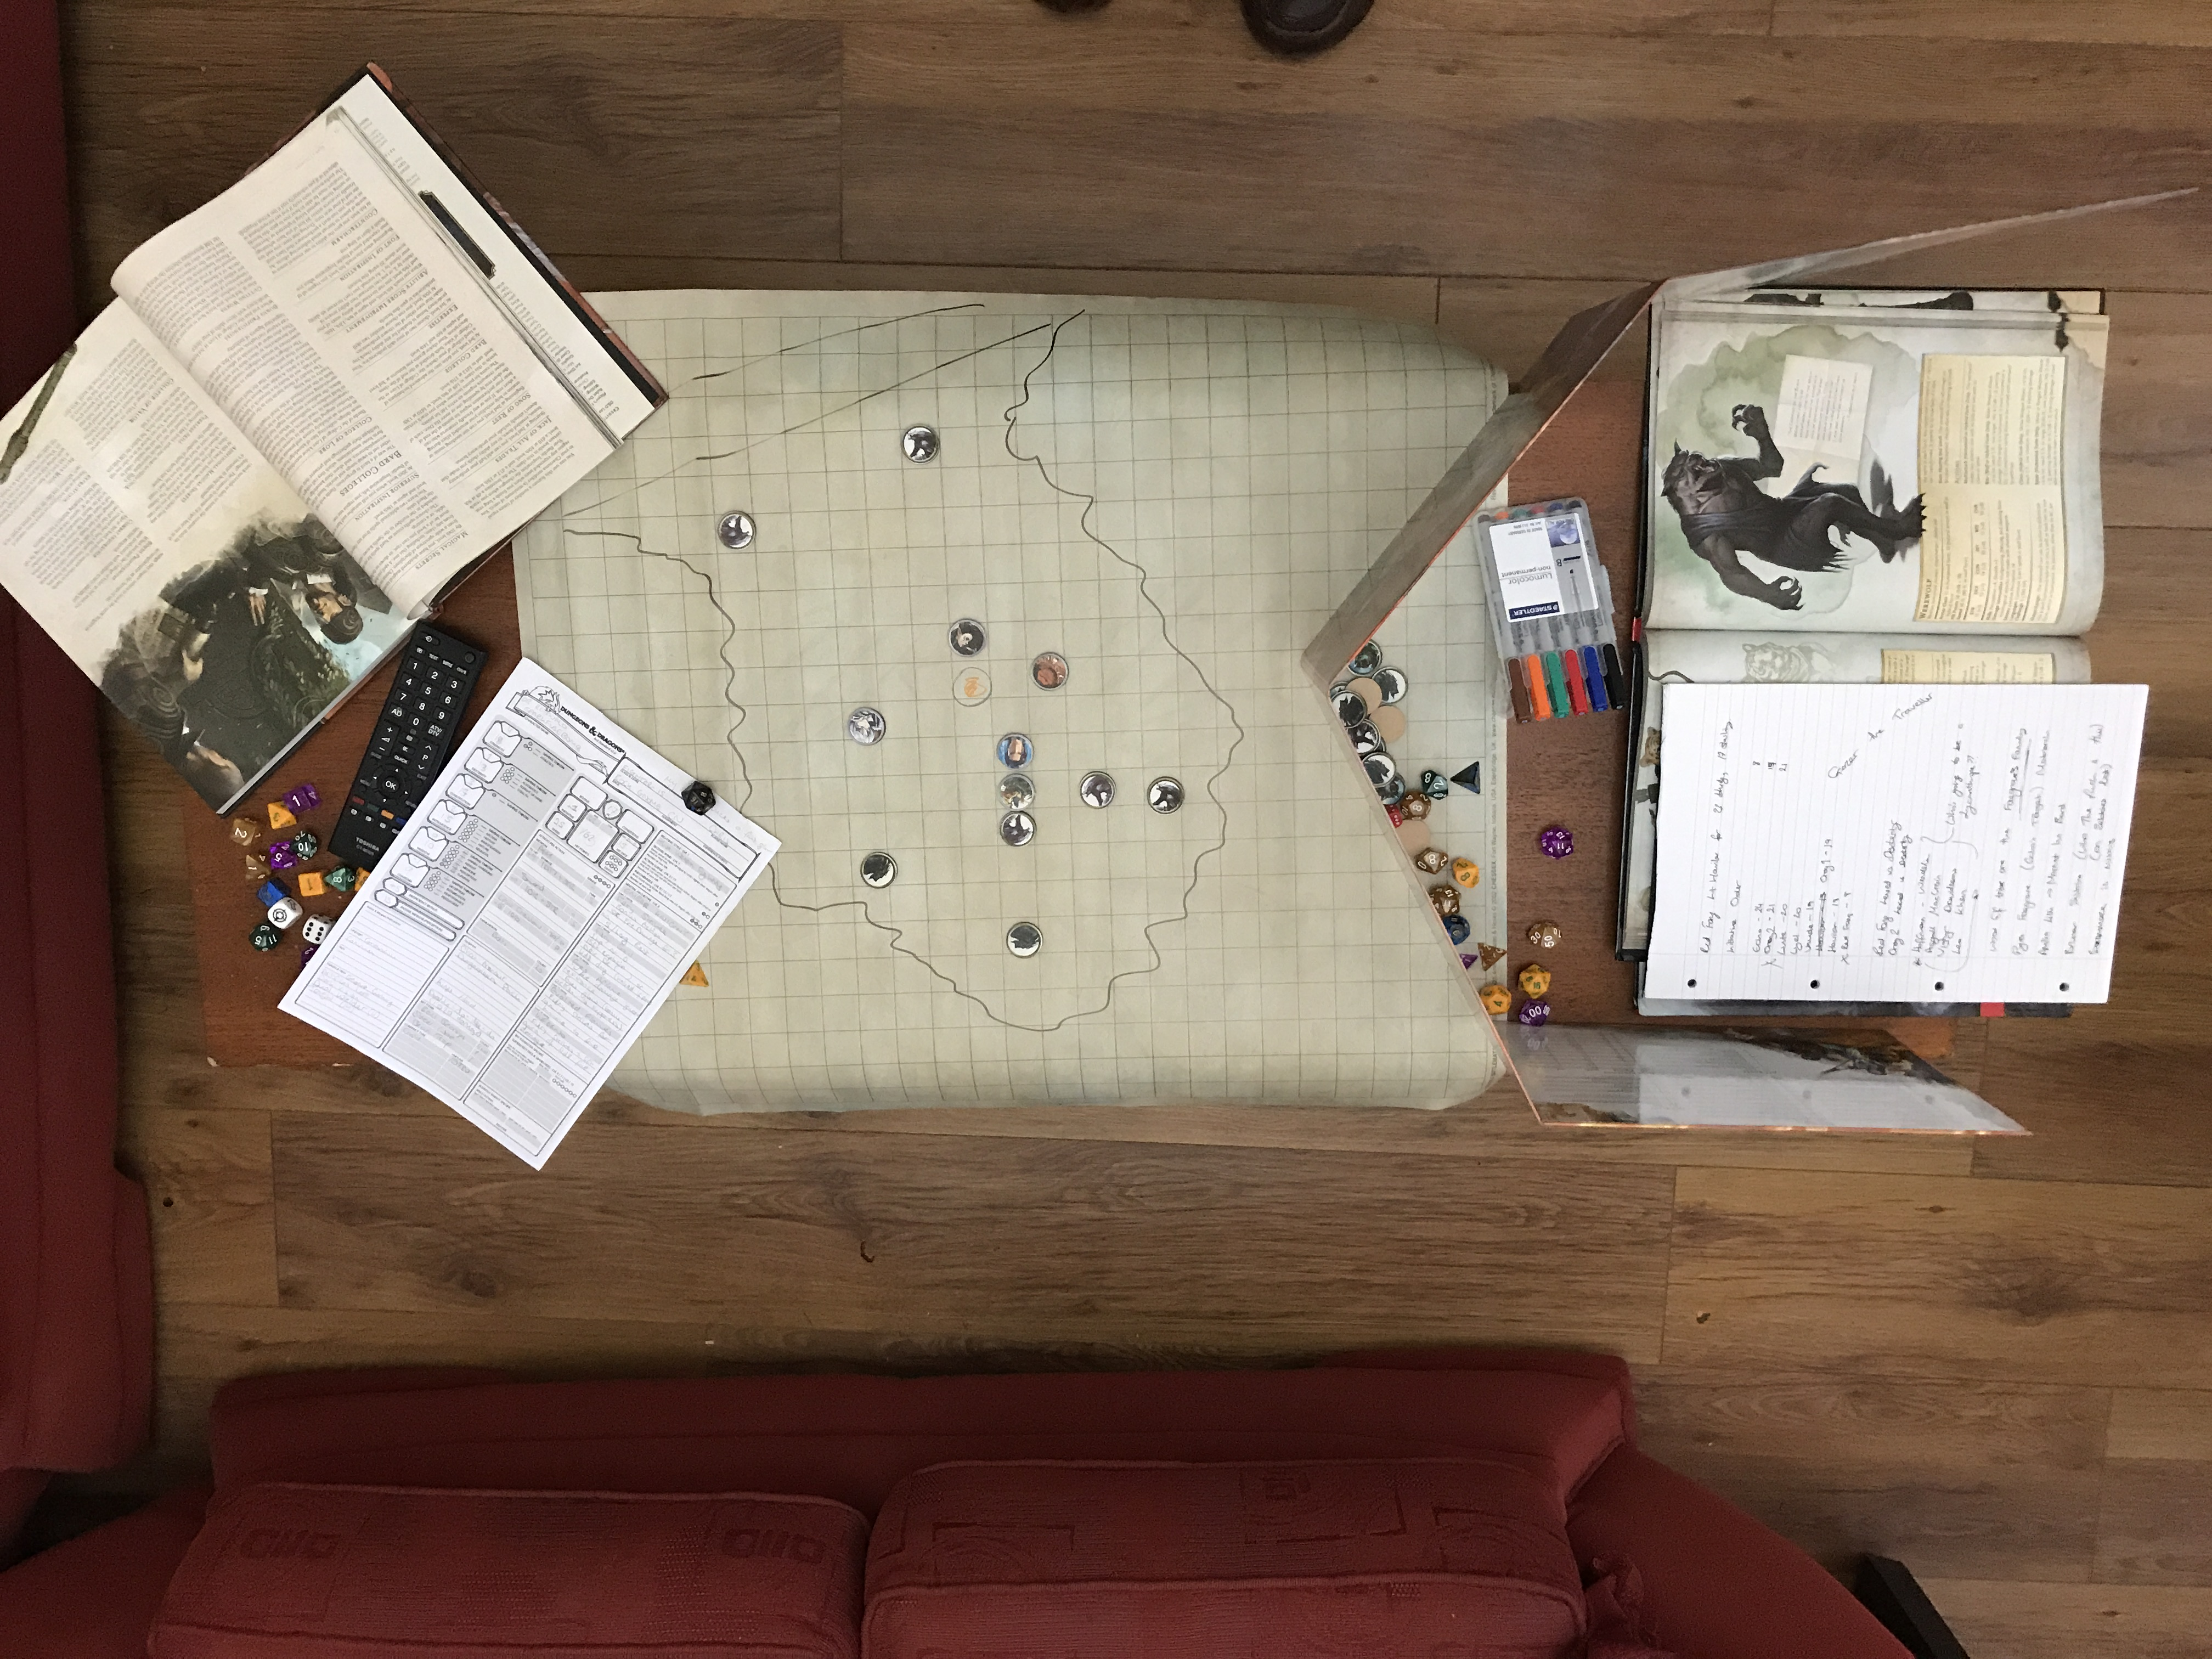
\includegraphics[width=\linewidth, height=5cm, angle=180]{DnD_Live.jpg}
					\caption{A typical \dnd \ set up. From left to right: DM note pad on top of a couple of official \WotC \ core books (\emph{Monster Manual} shown), set of dice, battle mat and tokens, a player character sheet, player's set of dice and the \WotC \ \emph{Players Handbook}} \label{fig:DnDLive}
				\end{subfigure}
				\begin{subfigure}{0.5\textwidth}
					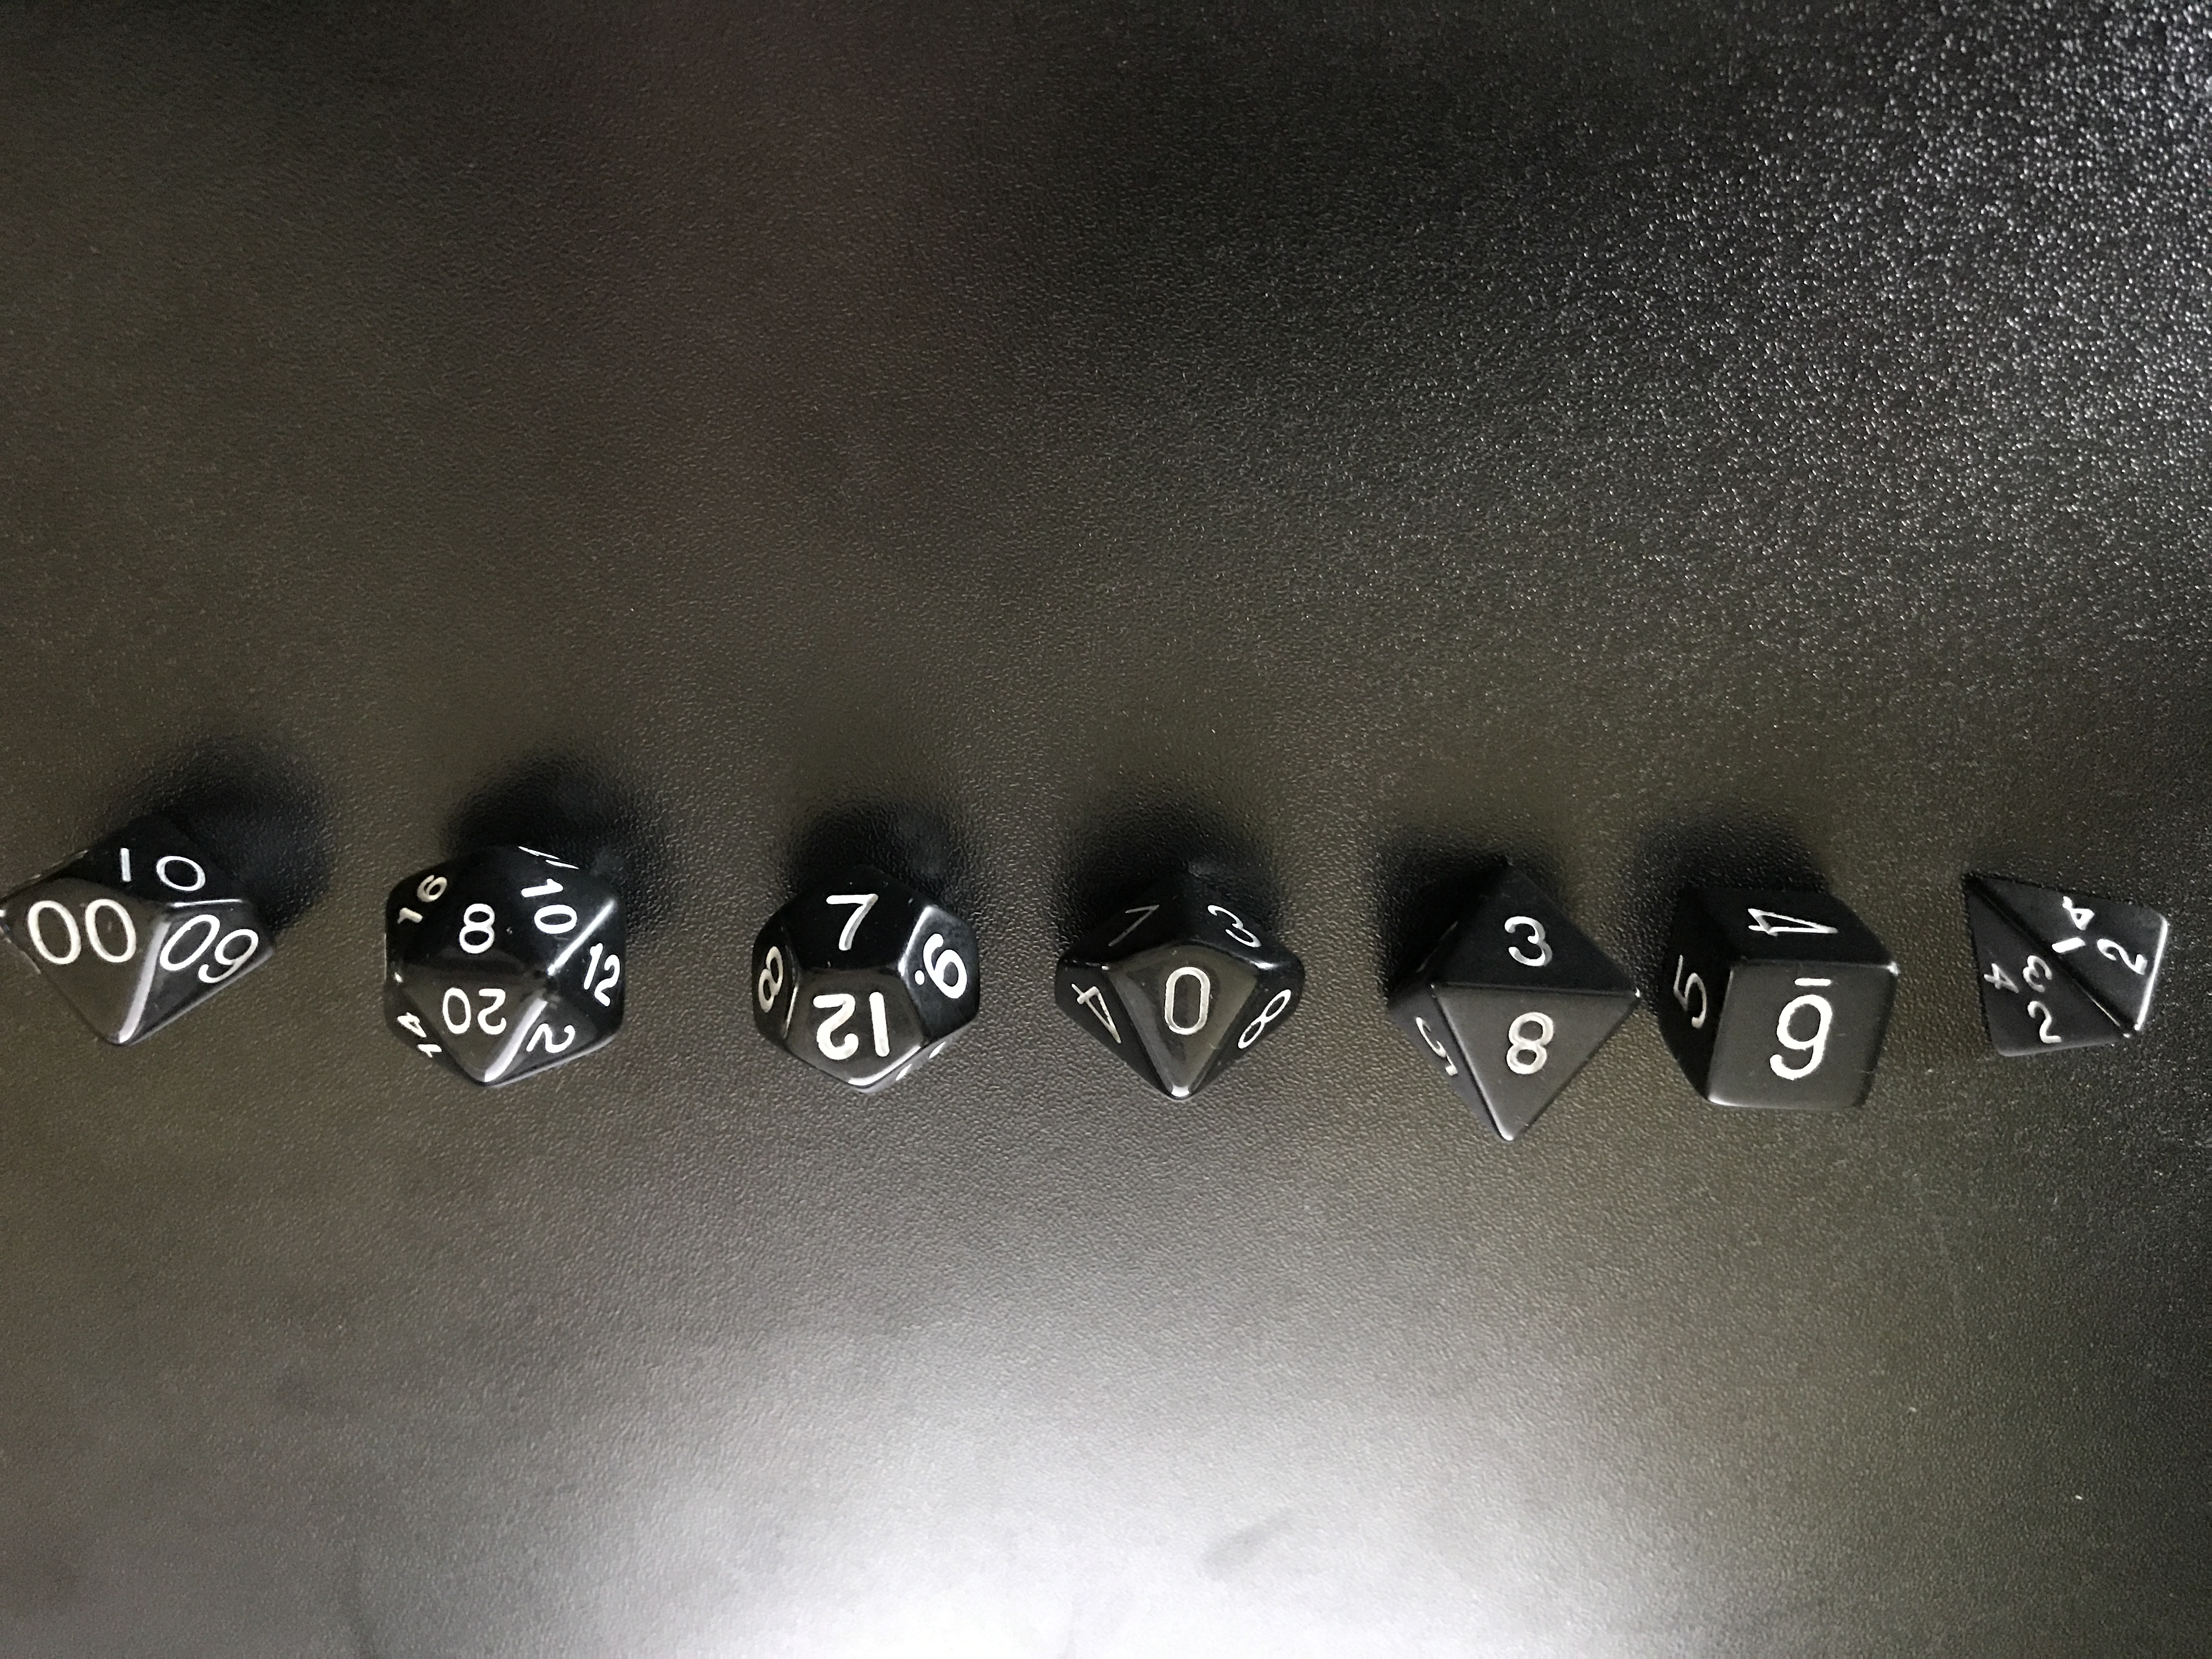
\includegraphics[width=\linewidth, height=5cm, angle=180]{DnD_Dice.jpg}
					\caption{An example set of dice that was needed to play \dnd. From left to right: 4-sided, 6-sided, 8-sided, 10-sided, 12-sided, 20-sided and a 10-sided dice in increments of 10s} \label{fig:DnDDice}
				\end{subfigure}
				\caption{Examples of the typical equipment used in a game of \dnd.} \label{fig:dnd-equipment}
			\end{figure}
			
			Despite the complicated nature of \dnd \ the equipment that was needed to play the game was minimal. A group of players would only have needed a single set of dice, a copy of the core books (\emph{Dungeon Master's Guide \citep{DMGuide}, Players Handbook and Monster Manual \citep{MonsterManual}}), a set of character sheets (1 per player), pens and paper. Everything else, such as more dice, a \emph{Dungeon Master Screen}, Campaign Books, Battle Mats and Tokens were supplementary. The dice that was used for \dnd are as follows; twenty-sided, twelve-sided, two ten-sided (one in increments of ten, the other in increments of one), eight-sided, six-sided and four-sided. Figure \ref{fig:DnDLive} is an example of what a \dnd \ table might have looked like, whereas Figure \ref{fig:DnDDice} is an example of the different dice used for \dnd \footnote{When discussing these dice further in this paper, they will be referred to as d\emph{X} where \emph{X} is the number of sides the dice has (for example the 20 sided dice is referred to as \emph{d20}). The exception to this is the secondary d10 (which has increments of 10) which is referred to as the \emph{d100}.}.
			
			Throughout the campaign the party would have to face many challenges designed by the DM. These challenges might be full scale battles involving multiple powerful enemies and allies, to small scale skirmishes between only a handful of characters. Alternatively challenges could be a battle of the wills where the party have to negotiate themselves out of a tight situation with the law to passing through a magical trap set by an ancient being in order to acquire an item of treasure. The effectiveness in which the party would handle these situations are decided through a simple mathematical system. 
			
			Every character within a \dnd \ world had a set of \emph{attributes} that would dictate how that character interacted with the environment around them. These attributes are; \emph{strength}, \emph{dexterity}, \emph{constitution}, \emph{intelligence}, \emph{wisdom} and \emph{charisma} (more details of these attributes are available in Appendix \ref{app:worked-example}). These attributes were rated between 1 and 20, with 20 being the highest a character could achieve without magical means. The score would be divided by 10, rounding up to the nearest whole number, creating an \emph{ability modifier} which would be applied to the role a dice (this number could be negative) If a character was highly skilled in a particular task, then a \emph{proficiency bonus} would also be applied. This calculation is summarised in the below equation \ref{eq:skill-check}. 
			
			\begin{equation} \label{eq:skill-check}
			skill \ check = d20 + ability \ modifier + proficiency \ bonus
			\end{equation}
			
			These skill checks allowed the players to interact with the world, via the player character, in a quantitative manner. The higher a skill check was the better that character performed in that challenge. Challenges would have a \emph{difficulty class}, an arbitrary number which indicates the level of skill (or luck in some cases) needed to perform that task. If the challenge was to strike an enemy, it would be easier to wound someone wearing no armour than it was to wound a skilled warrior in plate armour. 
			
			Winning a game of \dnd \ was no simple manner either, as there were no set win conditions. It depended entirely on the campaign that was being ran by the DM. A typical example might be that the party were a group of loyalists who were tasked with overthrowing a usurper and restoring the rightful monarch to the throne. That party would \emph{win} where they to do so, however the objectives might change where the party to learn of some new, unsavoury, information about their beloved monarch. A campaign might end without achieving the original goal, or shorter campaigns may end with the start of a new story for the party. It all depended on the attitude of the players towards the game.
			
			For a short, worked example of \dnd \ please refer to Appendix \ref{app:worked-example}, where a scenario is explored and explained. 
			
			\subsubsection{How does a Dungeon Master differ from a Player?} \label{sec:dm-vs-player}
			In Section \ref{sec:what-dnd}, we explored some of the principles that gave \dnd \ life, however the most important principle to the \Codex \ app was the difference between a DMs and Players. As briefly explained above, a DM was a member of the group who would control the narrative of the campaign and dictate what was occurring during each session. Whilst the DM may write the campaign narrative themselves and would of had a great deal of control over it, they would not own the story. That belong to the group as a whole. Player input during the sessions shaped the world and story as the party progressed through the campaign, forming relationships with characters that the DM portrayed. 
			
			It was the responsibility of a DM that the party was enjoying the campaign, narrative and challenges. As a result the DM would had to have known every intricacy of the world at any given time, or be able to improvise when they did not know the answer. Only a DM could bring a world to life. Therefore the amount of information that a DM would have to deal with would have been immense. Every DM would have a folder (either physical or digital) full of notes on places, people and events that resided within the DMs world. This folder would not only contain the events of the past, but plans for the future. Skilled DMs would rely on their folder more than any other resource during a session to ensure the correct reaction to party input. The maintenance of a DM folder was costly in both time and effort \citep{GMTips}. Whilst there was no definitive time spent in order to prepare for a session, DMs could easily spend over ten hours a week planning their \dnd \ campaign \citep{DungeonMaster}. 
			
			However, DMs were part of the game just like the players were. \dnd \ was never the party against the DM, instead it was a symbiotic relationship where they would explore the world together and share the experience. Whilst a DM knew what was planned to happen next, it was decided by the players if what actually occurred. 
				
			\subsubsection{Why was the \Codex \ app developed?} \label{sec:why-codex}
			As mentioned in Section \ref{sec:context}, \Codex \ began as personal project for the author of this paper. The original functionality of the app was to be a platform for tracking combat during games of \dnd. Since then the functionality has grown to include a note taking system and several other minor features that will be discussed in Section \ref{sec:dev-and-imp}. Whilst there are several other systems (explored Section \ref{sec:other-dnd-apps}) that assist a DM, they often only perform one task. The \Codex \ app aimed to be the assistance app for DMs by possessing a wide range of functionality. 
			
			DMs spend a lot of time and effort in running their games of \dnd (as discussed in Section \ref{sec:dm-vs-player}). The \Codex \ app attempted to remove some of the more laborious tasks from DMs and put more enjoyment into the game by removing some of the pressure. As of the time of writing, the principle functionality the \Codex \ app was to track combat and provide an interactive database of information about the world for quick reference.

	\section{Related Work} \label{sec:related}
	In this Section we will explore the work that was pertinent to the \Codex \ project. We will have a greater appreciation of the \Codex \ app, by evaluating the similar systems available at the time of writing, and and gain an understanding of the Software Engineering discipline in addition to the Web-App architecture through the review of academic works.
	
		\subsection{Dungeon and Dragons Apps} \label{sec:other-dnd-apps}
		At the time writing, there were several applications that existed to assist in the running of \dnd. These apps had varying levels of functionality, however they differed from the \Codex \ app. For example, the official \dnd \ Beyond app \citep{dnd-beyond} (discussed further in Section \ref{sec:dnd-beyond}), had a huge range of functionality including digital character sheets and a quick reference database. This service is aimed towards the players of the game, not towards the DMs, therefore \dnd \ Beyond does not support session planning and encounter generation to the same level as the \Codex \ app.
		
			\subsubsection{\dnd \ Beyond} \label{sec:dnd-beyond}
			\dnd \ Beyond was a web app that was developed by \emph{Curse, Inc.} and published by \WotC \ (the creators and owners of \dnd). The purpose of \dnd \ Beyond was to digitise the experience of \dnd \ without removing the table-top, social aspect (see Section \ref{sec:roll20}). However, \dnd \ Beyond was not just a web-app that held digital records of a User's character. There was an additional emphasis on community and sharing between the Users through the use of Forums and the ability to publish individual content through the site. 
			
			\begin{figure}[H]
				\centering
				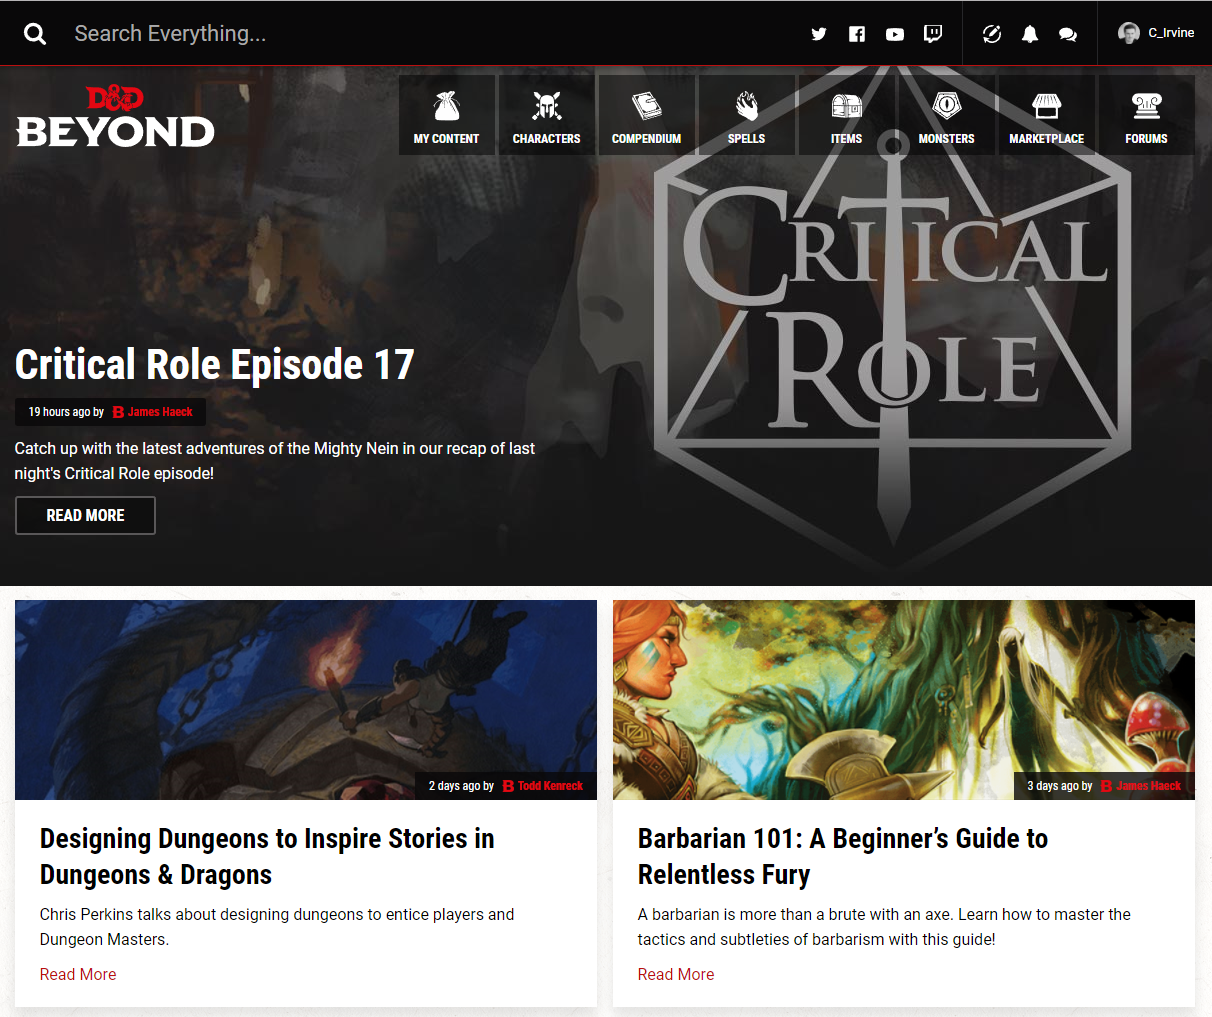
\includegraphics[width=\linewidth]{dnd-beyond.png}
				\caption[\dnd \ Beyond hompage screenshot]{A screen shot of the \dnd \ Beyond web-app homepage (05/05/2018), showing the various functionality of the service. We can see several articles (with more off-screen); separate sections for personal content, characters, compendium (campaign section), spells (see the Extended \dnd \ Explanation in portfolio for more details on spells), items, monsters, marketplace (where users may purchase electronic books to unlock content) and forums in the navigation bar. Additionally there is search, social media, chat and account functionality in the header of the screenshot.} \label{fig:dnd-beyond}
			\end{figure}
		
			Figure \ref{fig:dnd-beyond} is a screenshot taken from the \dnd \ Beyond homepage. Whilst a full description of the functionality of \dnd \ Beyond is available in the Design Document held within the project portfolio, we should understand some of the key features of the service. Firstly, the ability of digitally store a character, with a full description of abilities and spells attached to that character was critical to many players, who were frustrated at the constant searching through the core rule books of the game frustrating. Secondly, \dnd \ Beyond gave the community the ability to directly share and use content created not by \WotC \ but by other players of the game. Whilst this was happening on alternative sites such as the Reddit \dnd \ Forum \citep{reddit-dnd} (a popular forum website), \dnd \ Beyond brought the community back to \WotC \ and centralised it. However, one of the largest downfalls of \dnd \ Beyond was the compulsion to purchase the \WotC \ books through the web-app, even if the user might own a physical copy already. Only by purchasing the book (potentially for a second time) could the user access the majority of the content on the web-app (see Figure \ref{fig:dnd-beyond-mm}).
			
			\begin{figure}[h] 
				\begin{subfigure}{0.5\textwidth}
					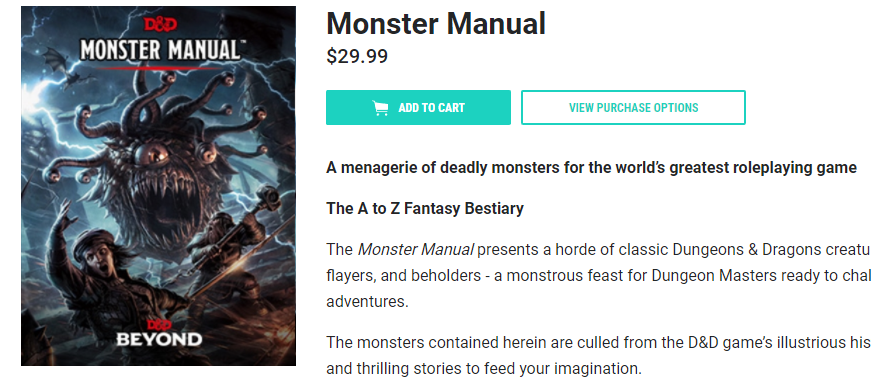
\includegraphics[width=\linewidth]{dnd-beyond-mm-purchase.png}
					\caption{\dnd \ Beyond \emph{Monster Manual}} \label{fig:dnd-beyond-mm}
				\end{subfigure}
				\begin{subfigure}{0.5\textwidth}
					
\includegraphics[width=\linewidth]{roll20-mm-purchase.png}
					\caption{Roll20 \emph{Monster Manual}} \label{fig:roll20-mm}
				\end{subfigure}
				\caption[\dnd \ Beyond and Roll20 Comparison Screenshots]{Screenshot taken from the \dnd \ Beyond and Roll20 web-apps showing the option to purchase a digital copy of the \emph{Monster Manual}, unlocking the relevant content} \label{fig:mm-purchases}
			\end{figure} 
			
			\subsubsection{Roll20} \label{sec:roll20}
			\begin{figure}[h]
				\centering
				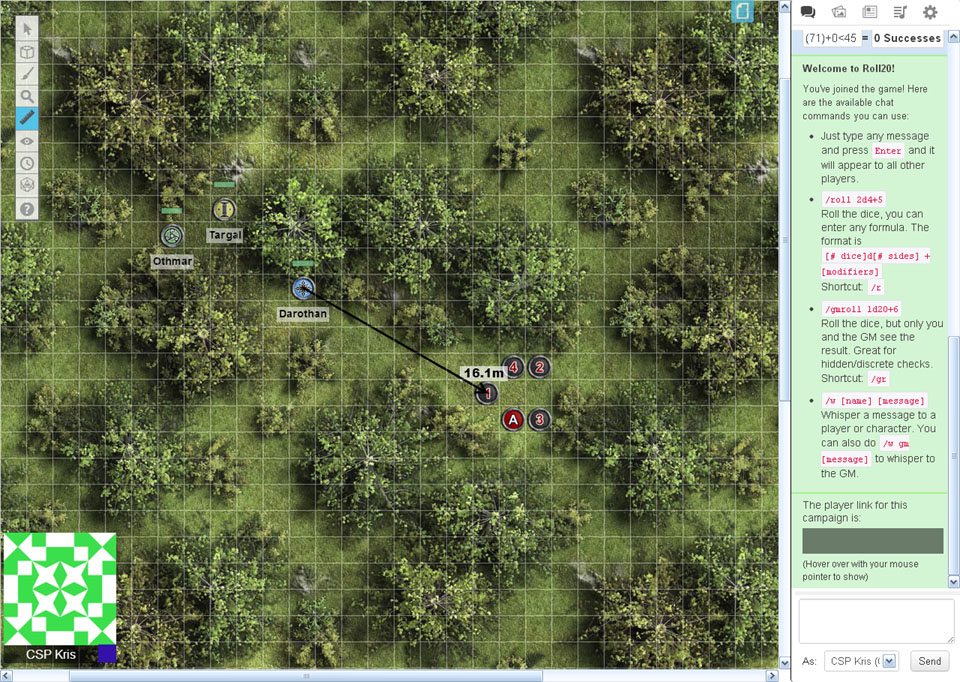
\includegraphics[width=0.75\linewidth]{roll20-example.jpg}
				\caption[Roll20 Screenshot]{A screenshot taken from the Roll20 web-app showing the table-top, text and voice chat functionality \citep{roll20-example}.} \label{fig:roll20}
			\end{figure}
		
			Roll20 \citep{roll20} was a popular web-app that was developed to enable games of \dnd \ to function without the need of a group of people coming together at a table. Instead, the group would use Voice over IP (VoIP) technologies (such as Skype or Roll20's internal VoIP system) to communicate and the Roll20 app would serve as the gaming table (see Figure \ref{fig:DnDLive}). 			
			
			Figure \ref{fig:roll20} shows a typical Roll20 virtual table-top in use. In comparison, we can see that the grid in the screenshot is very similar to the battle mat shown in Figure \ref{fig:DnDLive}. The DM of a group can use Roll20 to plan encounters and scenes for the party, and illustrate certain points to greater effect than at a physical table. All dice rolling can be performed from the Roll20 chat system, with graphical dice rolling across the virtual table-top. Without the Roll20 web-app some groups would not be able to function. However, for some groups the removal of the personal touch of meeting in person was not acceptable. 
					
			Roll20 was more than just a virtual table-top, as a quick reference database could be accessed through the purchase of \WotC \ books in a similar manner to \dnd \ Beyond (see Section \ref{sec:dnd-beyond}), as demonstrated in Figure \ref{fig:mm-purchases}. 
			
			\subsubsection{Kobold Fight Club} \label{sec:kfc}
			\begin{figure}
				\centering
				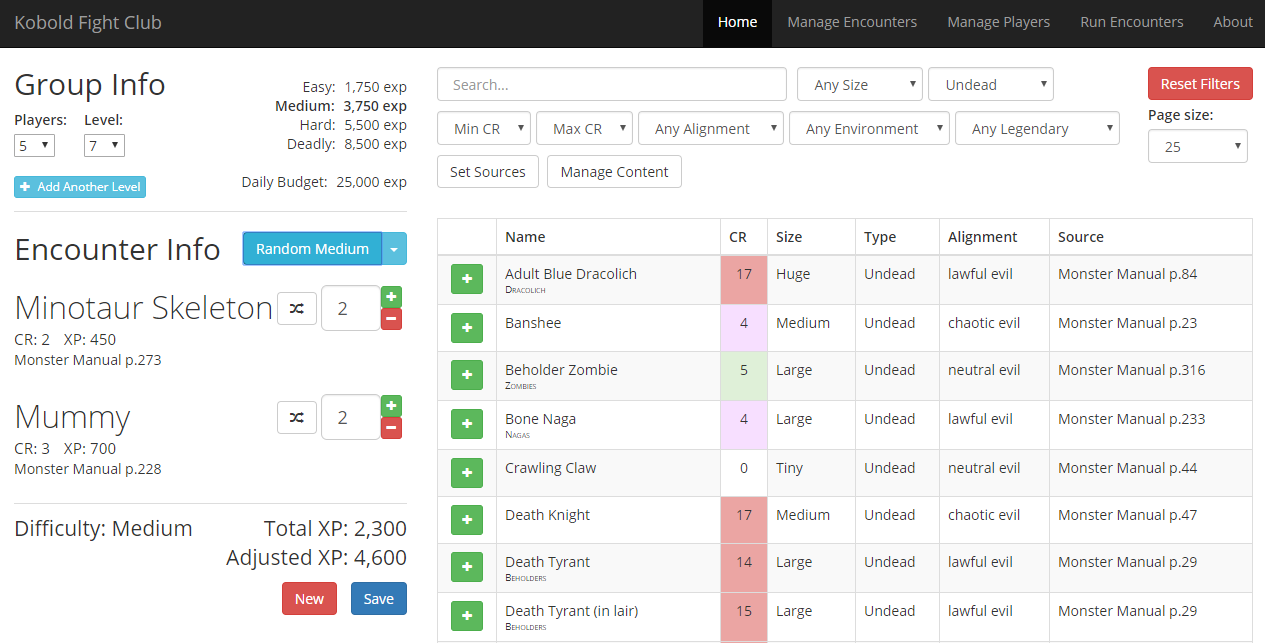
\includegraphics[width=0.8\linewidth]{kfc-screenshot.png}
				\caption[Kobold Fight Club Screenshot]{A screenshot showing an encounter designed using the Kobold Fight Club website, a popular \dnd \ encounter building tool}\label{fig:kfc}
			\end{figure}
			
			
			Kobold Fight Club (KFC) \citep{kfc-homepage}, named after one of most popular monsters in \dnd, was a website that assisted many DMs in creating and balancing encounters with enemies during a campaign. KFC only had a single function at the time of writing, which was the encounter planning. KFC was an example of a website that provided a single service to an excellent standard with a clean UI that was easily understood, as shown in Figure \ref{fig:kfc}. KFC does have some weaknesses, in order to make the service free and open to all the developers could not include the attributes of each monster. Instead they can only provide a page reference for that monster.
	
		\subsection{Software Engineering} \label{sec:software-eng}
		The \Codex \ project was not only the development of a web-app based around the \dnd \ game. It was the evaluation and examination of an agile single developer software engineering methodology. In order to perform this evaluation, we must first have an understanding for the Software Engineering Discipline (see Section \ref{sec:what-se}). From there we will learn about the Agile principles and how they changed Software Engineering (see Section \ref{sec:what-agile}). Finally, we will examine two potential single developer agile methodologies which would be compatible with the development of the \Codex \ app (see Sections \ref{sec:agile-solo} and \ref{sec:xp-for-one}). 
			
			\subsubsection{What is Software Engineering?} \label{sec:what-se}
			As stated multiple times throughout this paper, \Codex \ was not only the development of the \Codex \ app. \Codex \ aimed to evaluate an agile software engineering methodology that was suitable towards the single developer. In this subsection we will learn what Software Engineering was, at the time of writing, before gaining an understanding of the Agile Principles (see Section \ref{sec:what-agile}). 
			
			\begin{displayquote}
				"The systematic application of scientific and technical knowledge, methods and experience to the design, implementation, testing and documentation of software." -- \cite{SE-def}
			\end{displayquote}
		
			As explained in the definition above, Software Engineering was application of engineering practices to the development of Software, in order to produce the best Software solution to the proposed problem. These practices were reduced down to a series of stages that each project would be expected to progress through at least once during the project life cycle. Software Engineering is applied to a project is through Software Engineering Methodologies (SEMs). Please note that these stages may have different names depending on the selected SEM, however generally they were known as:
			
			\begin{itemize}
				\item Requirements analysis
				\item System Design
				\item Implementation or Development
				\item Testing
				\item Deployment
				\item Maintenance				
			\end{itemize}
		
			\emph{Requirements analysis} (sometimes called requirements engineering) was when a developer (or team of developers) would discuss the problem with the client in order to create a well defined list of requirements that a potential software system would need to fulfil in order to be a success. Later that list would be prioritised into four lists using a MoSCoW analysis (see Section \ref{sec:design} for the \Codex \ MoSCoW analysis). Those lists being must have, should have, could have, won't have. Several other investigative techniques may be used during the requirements analysis stage of a project, sometimes referred to as \emph{Systems Analysis}, such as Rich Pictures and Stakeholder wheels. By the end of a requirements analysis stage the project will have a clear set of criteria that it has to meet in order to succeed.
			
			The \emph{System Design} stage was closely related to the requirements analysis stage, they were sometimes merged together by some methodologies. During this stage the developers would design the proposed software system. This does not only mean the graphical look of the system; but the architecture that organises the classes, the methods that populate them and how information is transferred to different parts of the system. This stage would produce a document known as the \emph{Design Document} (see Section \ref{sec:design}). This document would give future developers the information necessary to contribute towards the development of a system and would be regularly updated throughout each iteration of a project.
			
			During the \emph{implementation (or development)} stage of a project, the developers would build the system as designed from the previous stages. Depending on the SEM being used by the development team, there might be the ability to revisit the requirements and design stages in order to fix unforeseen design errors or adjust to changing client demands. 
			
			The \emph{testing} stage of a project may occur after or during the implementation stage, depending on the applied SEM. Developers who practised \emph{Test Driven Development} (TDD) would have a large base of automated tests that would check a large percentage of the code regularly \citep{TDD}. That percentage is known as \emph{code coverage}. Regardless of whether TDD was used during the implementation stage the developers would still have to test the system themselves. This testing would involve the developers attempting to find bugs and/or security issues with the system. Eventually letting individuals (such as prospective users or experts in software security) test the system in order to get feedback and different opinions on the current system. One such method of testing using these individuals might be a \emph{Think-Aloud Evaluation} \citep{thinkaloud}. Any issues found during this stage would be corrected by the developers \citep{testing}.
			
			The \emph{deployment} stage of a system would be a crucial step in any project. Developers had several processes to choose from when deploying their system; direct, parallel, phased or piloted distribution. Each has their own strengths and weaknesses. Different systems would benefit greater from different deployment processes. 
			
			Once a system has been deployed, the maintenance stage may begin. Whilst during this stage additional features may be implemented into the system, they would fall into a life cycle of their own. Maintenance stage activities are limited to the identification and correction of any errors within the system, and it would have no definitive time scale. As long as the system was running, regular maintenance would have to be performed.
						
			\begin{figure}[h]
				\centering
				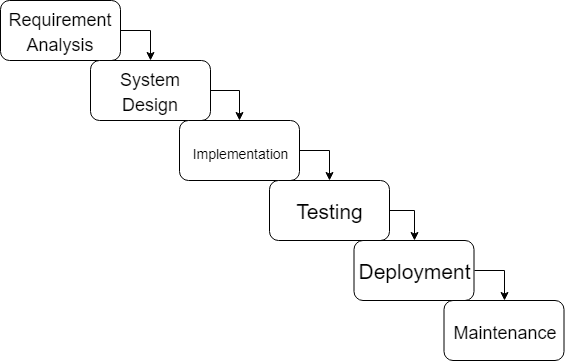
\includegraphics[width=0.8\linewidth]{waterfall.png}
				\caption[Waterfall Flow Diagram]{Flow Diagram showing the linear progression of a Waterfall Project.} \label{fig:waterfall}
			\end{figure}
			
			There are a variety of SEMs that have been tried and tested by several projects, with each possessing strengths and weaknesses. The earliest SEMs followed a \emph{Waterfall model}, where each stage would be completed in a linear sequence (see Figure \ref{fig:waterfall}. The popularity of Waterfall models arose from the simplicity they brought from a management view. The lack of iterations allowed a project manager to \emph{``cross off"} each section in sequence and move onto what was next. The industry would eventually realise that the rigid linearity of the Waterfall model prevented the developers adapting to changing client demands. 
			
			\begin{figure}
				\centering
				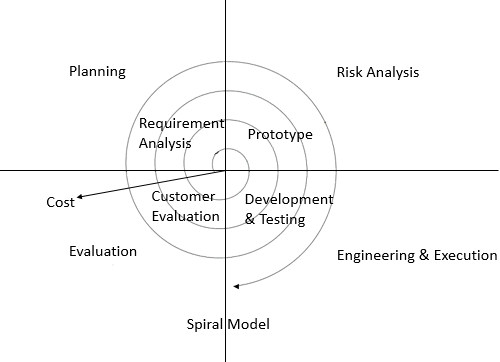
\includegraphics[width=0.8\linewidth]{spiral.png}
				\caption[Spiral Model Flow Diagram]{Flow Diagram showing the iterative design of the Spiral Model.} \label{fig:spiral}
			\end{figure}
			
			Iterative SEMs were created, such as \emph{Spiral Model}, that formed the basis for the Agile Principles to be created (see section \ref{sec:what-agile}). The Spiral Model, as seen in Figure \ref{fig:spiral}, follows an iterative design that condenses the system life cycle into four distinct phases: planning, risk analysis, engineering \& execution and evaluation. Within the planning phase the activities that were usually be associated with the requirements analysis and system design stages would be found. Risk analysis, an additional stage added by the Spiral Model, would ask the developer to prototype and examine the designed system to attempt to reduce the number of errors that would need fixing further into the project -- reducing costs. The engineering \& evaluation stage would see the approved system built and tested, before finally being deployed just prior to the evaluation stage where the users would provide feedback. That feedback was then incorporated into the next iteration of the project, where the spiral would begin anew.
			
			The \Codex \ app development has followed a methodology, discussed in Section \ref{sec:agile-solo} and was described as a software engineering project. This means that the development followed the systematic application of engineering practices, managed by the Agile Solo methodology.
				
			\subsubsection{What is Agile?} \label{sec:what-agile}
			Agile was a set of ideas and principles that would shape the way in which software was developed. The creators of Agile were frustrated with how software was built in the 1980 and 90s. Before Agile, a linear approach was taken (see Figure \ref{fig:waterfall}) towards software development. For example, once a set of requirements for a system was decided, it could not be changed because the project management could not allow it. Another frustration was the lengthy and complicated contracts that bound both client and developers to a proposed system. These are but a few frustrations that were felt by the creators of Agile, who wanted to ``\ldots uncover better ways of developing software \ldots" \citep{AgileManifesto}. 
			
			What was produced by the desire to produce better software was known as the \emph{Agile Manifesto}, at the core of which were four values:
			
			\begin{enumerate}
				\item \textbf{Individuals and interactions} over processes and tools
				\item \textbf{Working software} over comprehensive documentation
				\item \textbf{Customer collaboration} over contract negotiation
				\item \textbf{Responding to change} over following a plan 
			\end{enumerate}
		
			The Agile Manifesto additionally states ``That is, while there is value in the items on the right, we value the items on the left more.". This distinction is critical to Agile, as the creators recognised that the traditional software engineering methods held a value and a place in the future. However, change must be embraced in order to keep up with the demands of that same future.
			
			With the release of the Agile Manifesto, many iterative SEMs became more popular and replaced the linear waterfall models as the industry standards. Scrum and Kanban are two such SEMs. 
			
			The Scrum methodology was governed by a ``\ldots simple set of roles, responsibilities and meetings that never change." \citep{scrum-online}. The roles within a scrum team are \emph{Product Owner}, \emph{Scrum Master} and \emph{Team}. The Product Owner may be a client or an executive who guides the scrum master and the team towards creating the product that should be delivered. Technical expertise was not required and the Product Owner should not be involved in the management of the development process. The Scrum Master was the facilitator towards both the Team and Product Owner, meaning that this individual would remove any impediments preventing the progress of the project. Scrum Masters do not manage the Team however as the Team is utterly self managing. There were 3 to 6 members in a Scrum Team that would select the work to do every \emph{sprint} in a \emph{sprint planning meeting}. Teams would contain a mixture of professionals including but not limited to software engineers, architects and UI designers \citep{Scrum}. 
			
			\begin{figure}
				\centering
				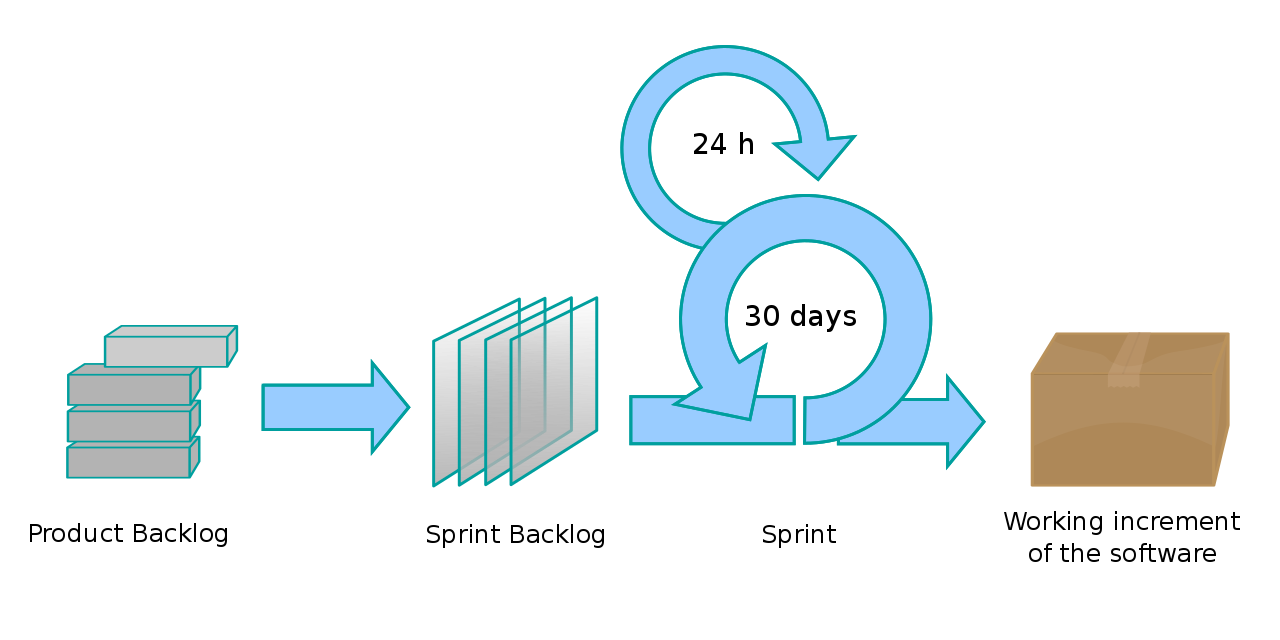
\includegraphics[width=0.8\linewidth]{scrum.png}
				\caption[Scrum Methodology Sprint Cycle]{Flow diagram detailing the stages of a Scrum \emph{sprint} cycle. At the beginning of each \emph{sprint} the Team and Scrum Master would select a set of tasks from the \emph{Product Backlog} and move them into the \emph{Sprint Backlog}. This occurs during the \emph{Sprint Planning Meeting}. During the 2-4 week \emph{sprint} the Team would progress through the \emph{Sprint Backlog} tasks, holding a tightly regulated short \emph{Scrum Meeting} daily. At the end of the \emph{sprint} the Team would have produced a potentially shippable increment of working software.} \label{fig:scrum}
			\end{figure}
		
			Scrum projects were organised into \emph{sprints}. At the beginning of each \emph{sprint} the Team and Scrum Master would select a set of tasks from the \emph{Product Backlog} and move them into the \emph{Sprint Backlog}. This occurs during the \emph{Sprint Planning Meeting}. During the 2-4 week \emph{sprint} the Team would progress through the \emph{Sprint Backlog} tasks, holding a tightly regulated short \emph{Scrum Meeting} daily. At the end of the \emph{sprint} the Team would have produced a potentially shippable increment of working software. This increment would be scrutinised in the \emph{Sprint Retrospective Meeting} which evaluated the work done, and any large scale issues would be solved before beginning the sprint anew with another \emph{Sprint Planning Meeting}.
			
			Whilst some projects would only use Scrum during the implementation stage of a project, perhaps within an iterative Spiral model (see Section \ref{sec:what-se} and Figure \ref{fig:spiral}), other project would choose to use Scrum throughout the project life cycle as to prevent confusion through the use of multiple different SEMs. 
			
			\begin{figure}
				\centering
				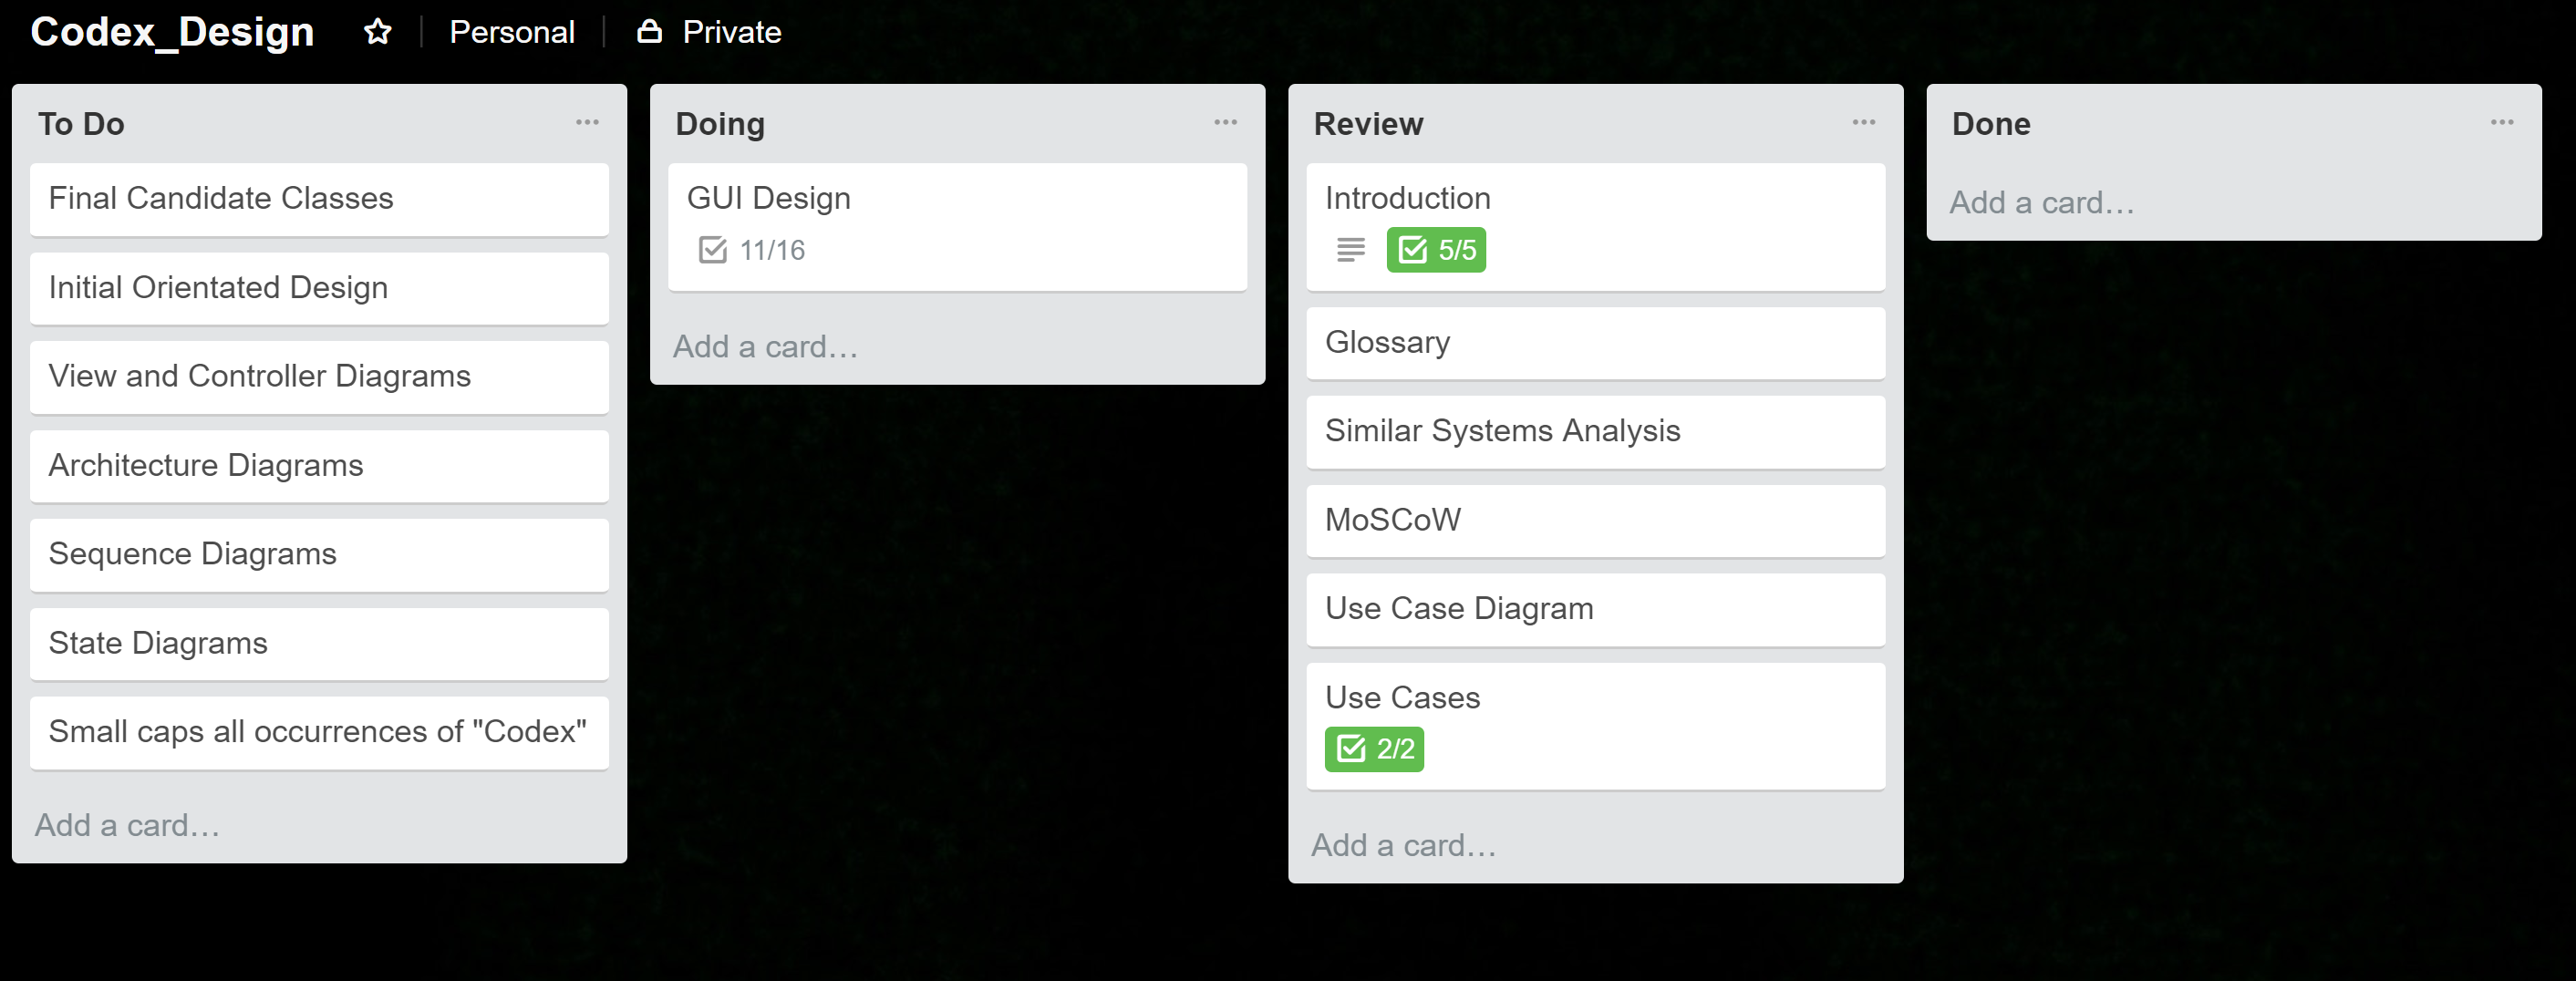
\includegraphics[width=0.8\linewidth]{trello_board.png}
				\caption[Example Kanban Board using Trello]{Screenshot taken from the early design stage of the \Codex \ app. Kanban Board developed using the Trello app \citep{trello} and includes an optional Review column.} \label{fig:kanban}
			\end{figure}
		
			Kanban was another popular Agile SEM, which whilst closely related to Scrum was a lean methodology rather than iterative. Despite this difference, Kanban was often used in conjunction with iterative SEMs, the most common being Scrum \citep{kanban}. Kanban was operated by balancing the demands of a project with the available capacity of the development team, with the ultimate goal of reducing the effect of system level bottlenecks. This was achieved through the use of a Kanban Board (see Figure \ref{fig:kanban}), which may have been either physical or digital. Kanban board must include the following columns: \emph{to do} (sometimes called Backlog), \emph{Doing} and \emph{Done} at a minimum. However, additional columns such as; \emph{plan}, \emph{test} (or review) and \emph{deploy} are recommended. The task \emph{tickets} would move from left to right through each of the columns on the board, eventually clearing the Backlog of tasks. Some users of Kanban might have colour coded tickets in accordance with different type of tasks; pink for development tasks and yellow for design tasks for example. Customisation of the tickets can be taken further when developers apply arbitrary levels of difficulty to the tickets in order to gauge the length of time taken to complete that task. 
			
			Kanban projects would not have to go through the regular planning that Scrum projects experiences, because Kanban project were not organised into Sprints. However, Scrum can benefit from the inclusion of Kanban boards to organise and manage the Product and Sprint backlogs.
			
			\subsubsection{Agile Solo} \label{sec:agile-solo}
			Agile Solo was a SEM developed by Anna Nystr{\"o}m in June 2011. The methodology was created using the values stated by the Agile Manifesto (see Section \ref{sec:what-agile}) and aimed to adapt the established working practices of existing Agile SEMs. However the definitive feature of Agile Solo is that the methodology was able to be implemented and used by a single developer. 
			
			Nystr{\"o}m selected the suitable components from many different existing Agile SEMs, such as the Sprint Cycle from Scrum (see Figure \ref{fig:scrum}), the Kanban Board (see Figure \ref{fig:kanban}) to name but a few. However, Nystr{\"o}m also realised that single developers rarely work in isolation as typically there would be a supervising individual assigned to the project and a client who would own the project, so adaptations were made to accommodate such individuals.
			
			\begin{figure}[H]
				\centering
				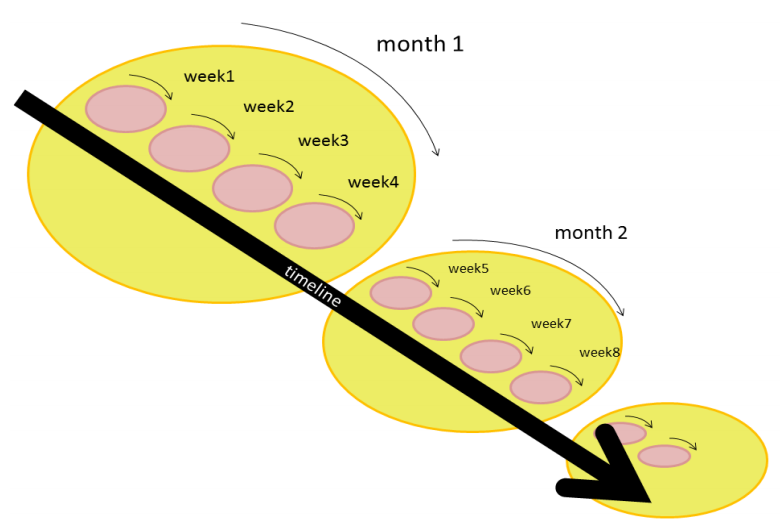
\includegraphics[width=0.8\linewidth]{agile-solo.png}
				\caption[Agile Solo Diagram]{Diagram to represent the Agile Solo Software Engineering Methodology. The project is segmented into \emph{monthly cycles} that would contain \emph{weekly sprints}. The developer would review the work done at the end of each sprint, with the customer and supervisors reviewing the work at the end of each cycle. The monthly cycle would begin anew with feedback from the customer and supervisor to be incorporated into the project.} \label{fig:agile-solo}
			\end{figure}
			
			The resulting methodology was called Agile Solo and revolved around monthly cycles with weekly sprint iterations. At the end of every sprint the developer would review and test the work done, whilst at the end of each cycle the customer and supervising figures would review and test the system providing feedback to be incorporated in the next cycle. This is demonstrated by Figure \ref{fig:agile-solo}. Nystr{\"o}m recommends that the product backlog should be managed by a Kanban Board and the software be implemented using Test Driven Development (TDD). 
			
			Agile Solo was selected to be the SEM for the development of the \Codex \ app (see Section \ref{sec:use-agile-solo}), and shall be evaluated later in this paper (see Sections \ref{sec:agile-solo-effect} and \ref{sec:agile-solo-eval})
			
			\subsubsection{XP for One} \label{sec:xp-for-one}
			Extreme Programming (XP) was a SEM which would attempt to improve the software quality through an iterative development loop that emphasised responsiveness to changing customer requirements. Typically paired with programming practices such as TDD and pairs programming, practitioners of XP believed that the only important product of development was code \citep{XP}.  
			
			\begin{figure}[H]
				\centering
				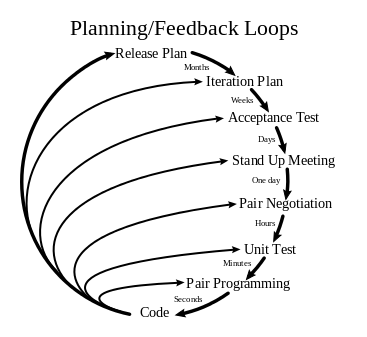
\includegraphics[width=0.6\linewidth]{xp.png}
				\caption[Extreme Programming Diagram]{Diagram to represent the Extreme Programming iterative life cycle.} \label{fig:xp}
			\end{figure}
			
			As seen in Figure \ref{fig:xp}, XP was highly iterative, with each task within the SEM having an iteration cycle. XP for One was an untested development methodology which had one critical difference from traditional XP, the removal of Pair Programming (pair negotiation in the diagram) \citep{SoloXP}. 
			
			In the event that Agile Solo (see Section \ref{sec:agile-solo}) was discovered to be unsuitable towards the development of the \Codex \ app, XP for One was to be the replacement SEM.
			
		\subsection{Web App Technology} \label{sec:web-app}
		The \Codex \ app was designed to be a Web Application (web app). In this Section we will learn what a web app is and how it differs from the traditional website and application (see Section \ref{sec:what-web-app}). ReactJS is a popular library for the JavaScript programming language that was developed specifically to develop web apps. Due to the popularity and availability of supplementary materials of ReactJS, it was selected to be the principle programming language for the \Codex App (see Section \ref{sec:react-js}). Semantic UI (User Interface) is a package developed for ReactJS systems, which would allow developers to quickly create professional UI for web apps and was used in the development of the \Codex \ app (see Section \ref{sec:semantic-ui}).
		
			\subsubsection{What is a Web App?} \label{sec:what-web-app}
			With the rising popularity of applications in the early 2000s, web developers understood the need to reinvigorate websites with new technologies to bring websites into the modern age. This resulted in the creation web-apps. A system that could operate as an separate application on a computer or mobile device, that could still be accessed through a browser (such as Google Chrome). Today web apps exist in between applications and websites \citep{web-apps}. 
			
			\begin{figure}[h]
				\centering
				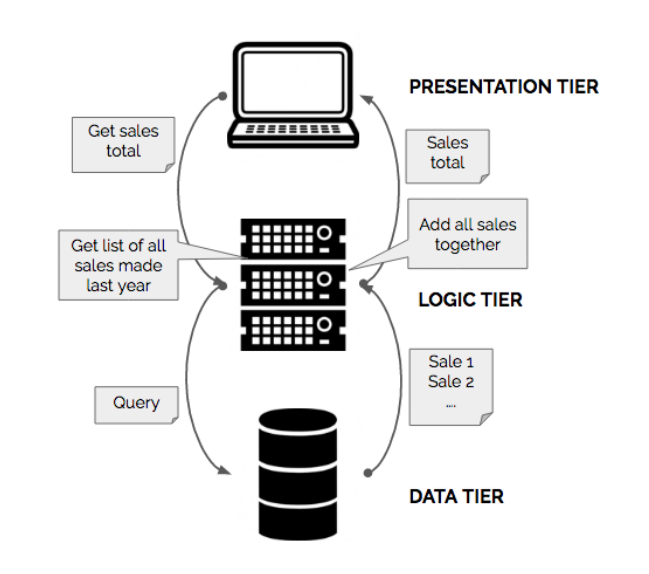
\includegraphics[width=0.5\textwidth]{Basic_Web_App_Architecture.PNG}
				\caption[Three Tiered Web App Architecture]{Diagram showing the flow of information between the three tiers of web app architecture. The \emph{presentation layer} allowed the user to interact with the system (and vice versa). The \emph{logic layer} would host the functionality of the system and generated the GUI. Finally the \emph{data tier} would hold the database that supported the web app.} \label{fig:web-apps}
			\end{figure}
		
			The \Codex \ web app will follow the web app three tiered architecture that was established with the technologies emergence. As we can see from Figure \ref{fig:web-apps} the first layer (Presentation Tier) is held locally on the Client's machine. This is what is known as `Client-Side'. Here HTML, CSS and JavaScript is used to translate data into a format the Client will understand. The second layer (Logic Tier), here languages such as ReactJS perform functions on raw data to generate web content. Traditionally the Logic Tier is hosted on a Server that Clients connect to, this is the `Server-Side' The third layer (Data Tier) communicates with the Logic Tier through SQL Queries \citep{SecurityWebApps}. 
			
			\subsubsection{ReactJS} \label{sec:react-js}
			ReactJS was a JavaScript library developed by Facebook, Inc. after the acquisition of Instagram \citep{ReactJSOfficial}. The library provided a set of components, and the ability to create components, that would be rendered by the ReactDOM. This allowed developers to quickly build user interfaces that were highly customisable without the use of traditional HTML components \citep{MasteringReact}. As ReactJS was developed around the JavaScript programming language there was pre-existing functionality support. This meant that entire websites and web apps could be developed in JavaScript and ReactJS (with a little CSS for styling). 
			
			The \Codex web app was developed using the ReactJS technologies, as it was one of the most popular web app languages available at the time of writing \citep{ReactJSPopularity}.  
			
			\subsubsection{Semantic UI} \label{sec:semantic-ui}
			One of the strengths of JavaScript technologies was the incorporation of \emph{open source packages} that would supply a programmer with a set of methods that could be called upon during development. The purpose of including packages instead of developing the methods personally is to save time and reduce costs. Packages allowed developers to focus on the more important tasks \citep{JavaScriptGuide}.
			
			Semantic UI was a package whose purpose was to provide a sophisticated set of UI elements and collections that can be easily styled through the use of CSS \citep{SemanticUI}. Many large organisations (Amazon, Netflix and Microsoft for example) had chosen the Semantic UI package to build their websites. The \Codex \ web app was developed using Semantic UI elements (see Section \ref{sec:codex-development}).
			
			
	\section{Development and Implementation} \label{sec:dev-and-imp}
	In this Section we will examine how the Agile Solo methodology (discussed in Section \ref{sec:agile-solo}) will be implemented into the \Codex \ project and later evaluated in Sections \ref{sec:agile-solo-effect} and \ref{sec:agile-solo-eval}. Next we will gain an understanding on the design of the \Codex \ web app through the extensive Design Document that can be found in the supporting materials. Finally, we will expand upon the knowledge gained in Sections \ref{sec:react-js} and \ref{sec:semantic-ui} to gain an appreciation of the development of the \Codex \ web app by dissecting some examples of source code.
	
		\subsection{Using Agile Solo} \label{sec:use-agile-solo}
		As explained in Section \ref{sec:agile-solo}, Agile Solo was centred around the idea of \textit{weekly sprints} encompassed by \textit{monthly cycles} (see Figure \ref{fig:agile-solo}. Whilst there was no recommendation by Nystr{\"o}m for the management of the project backlog, the \Codex \ implementation of Agile Solo will utilise the Product Backlog/Scrum Backlog system favoured by Scrum (see Section \ref{sec:what-agile}). At the end of each sprint the developer (the author of this paper) would test the \Codex \ system as it stood, in order to catch any issues that made it past the automated tests. A fortnightly meeting would be held with the supervisor of the project in order to ensure that the development of \Codex \ remained on track. At the end of each cycle the current state of the \Codex \ web app would be presented to a small group of users in order to ascertain the quality of the development done.
		
		The feedback generated from the supervisor and user meetings was stored within the project journal (found in the supporting material) and later incorporated into future developments, where possible. Also found in the journal, would be the initial evaluations and opinions of Agile Solo from the author of this paper as the development of the \Codex \ web app progressed. 
		
		\subsection{Design} \label{sec:design}
		The \Codex \ web app was designed through the creation of a Design Document \footnote{The \Codex \ Design Document can be found in the supporting material for this paper.}, which was briefly discussed in Section \ref{sec:what-se}. There we learned that a Design Document should contain a mixture of diagrams and analysis in order to convey to a new developer the design of a software system \citep{DesignDocExample}. These would include the analysis of requirements and similar systems. With diagrams to explain how the system was intended to be used, the GUI design, Class and Architecture Designs with optional additional diagrams that would demonstrate the flow of information throughout select use cases.
		
		The requirements analysis would consist of listing, in detail, the primary functions of the system. The \Codex \ Design Document elected to use bullet points in order to promote concise descriptions of the functionality. Bullet points additionally allowed the author of the Design Document to label certain functions as sub-functions. For example; the ``Account Creation" functionality has detailed under it that there should be ``Two `levels' of accounts - Player and Dungeon Master" within the system. From this detailed list a \emph{MoSCoW analysis} can be performed where the developer would designate which functionality was critical to the success of the system and which functionality would not be. MoSCoW contains four categories of functionality; Must Have, Should Have, Could Have and Won't Have. These categories would be organised into a table, that is shown in Table \ref{tab:moscow}.
		
		\begin{table}[h]
			\centering
			\begin{tabular}{|c|c|c|c|}
				\hline
				\textbf{Must have} 					& \textbf{Should have}              	& \textbf{Could have} & \textbf{Won't have}             	  \\ \hhline{|=|=|=|=|}
				Track Combat      					&\makecell{Multiple Campaigns \\ per DM Account}	& \makecell{Game \\ Scheduling}     & \makecell{Full descriptions of \\ D\&D} \\ \hline
				Accounts          					& Settings								& Items               & \makecell{Pre-made Settings \\ \& Campaigns}\\ \hline
				Encounter Planning 					& Characters                        	&                     & \makecell{Inter-account Direct \\ Messaging} \\ \hline
				Random Encounters  					& WorldWiki                        		&                     &                                	  \\ \hline
				Populated Database 					& \makecell{Run, Save \& \\ Delete Games} 			&                     &                                   \\ \hline
				Session Planning					&         								&                     &                                   \\ \hline
			\end{tabular}
			\caption[\Codex \ MoSCoW analysis]{MoSCoW analysis for \Codex, showing the differing importance of wanted features to the system as a whole. The \emph{Minimum Viable Product}(MVP) for the project is derived from the \emph{Must have} column. The \emph{Should have} column represents what features \Codex \ should contain for the system to be complete. The \emph{Could have} is what features might give \Codex \ an edge over similar systems and what would be ``nice to have''. Finally the \emph{Won't have} column represents what features will never be part of the \Codex \ system.}\label{tab:moscow}
		\end{table}
	
		The \emph{Similar System} analysis was a vital step for Design Documents, particularly the \Codex \ app, as it would ensure that the developer was not creating a duplicate for a system that already existed. Therefore, for commercial systems, this analysis may be seen as a form of risk assessment. Typically the findings of the Similar Systems analysis are stored within a table in the early stages of the Design Document. Sections \ref{sec:dnd-beyond}, \ref{sec:roll20} and \ref{sec:kfc} informed by the findings from the \Codex \ Similar Systems analysis. 
		
		Another key component of a Design Document would be the \emph{Glossary of Terms}, which would inform future developers of the terms required to understand the software system. The terms contained within this glossary would not extend to technical terms, unless they were uncommon at the time of development. Instead the glossary would focus on the contextual terms, in the case of \Codex \ the majority of the terms were \dnd \ related. The full glossary of terms for the \Codex \ app can be found in the Design Document.
		
		For every function detailed by the Design Document, there would be an accompanying \emph{Textual Use Case} and \emph{Use Case Table} which were then summarised into a \emph{Use Case Diagram}. The Use Case Diagram would show the authorisation that each type of user would have within the system. In the case of \Codex \ we have two types of users -- players and DMs -- and each had two levels of access to the system functions. Also shown by the Use Case Diagram is which use cases relationships: \emph{include} (meaning they are a prerequisite to) and \emph{extends} (which represents optional behaviours between use cases). See Figure \ref{fig:use-case-diag} for the Codex Use Case Diagram. The textual use cases and use case tables detail exactly how each function of the app would be used by the user. These details included goals, scope, triggers, end conditions, success and alternative scenarios to name but a few. The developer would study the use cases in order to gain an understanding of what the source code needs to reflect prior to starting development.

		The Graphical User Interface (GUI) design of the \Codex \ web app began with \emph{lo-fi prototyping}, where the developer would roughly sketch the design of the GUI and then quickly receive feedback from prospective users. With the feedback incorporated into the design, the lo-fi prototypes were transformed into \emph{hi-fi prototypes} by creating digital sketches using software. The \Codex \ web app GUI was designed using MarvelApp \citep{marvelapp}, which had a range of tools and allowed the prototyping of colour schemes and icons to be effectively tested. The hi-fi prototypes were shown to prospective users to gather feedback, who reported that the colour scheme was too dark. With the lighter palette integrated into the app, the GUI design was finalised and inserted into the Design Document as images. 
		
		Once the use cases and functionality of a system has been decided, the developer could now start allocating the functionality to classes within the source code. This was done through the Class Diagram, which shows the flow of information between the classes that divide the source code. Each class within the diagram would have the class and method names. The method names were designed to be self-explanatory to the developer. This was done so that when the developer was writing the source code, the Class Diagram could be referenced so that development would stay on track and the scope of the project would not creep \footnote{\emph{Scope Creep} is a term used by Software Engineers when the Scope (the functionality) of a system was extending (creeping) past the original parameters of the system in an unplanned fashion.} 
		
		The classes generated from the Class Diagram would be inserted into the Architecture Diagram, to create a graphical representation of the system architecture. Each class was allocated into one of the three tiers of the web app architecture (described in Section \ref{sec:web-app} and Figure \ref{fig:web-apps}): Presentation, Logic and Data. Similar to the Class Diagram, the Architecture Diagram guided the developer during the development process to ensure that each class was performing the tasks allocated during the design process. 
		
		\subsection{Development of \Codex} \label{sec:codex-development}
		The development of the \Codex web app was scheduled to take 9 weeks (see Figure \ref{gantt:pplan}), which allowed for multiple revisions of the design and development in addition to the writing and evaluation necessary for the project. 
		
		As mentioned in Section \ref{sec:web-app}, the \Codex \ web app was built using ReactJS (see Section \ref{sec:react-js}) with assistance from the Semantic UI package (see Section \ref{sec:semantic-ui}). Before providing examples of the \Codex \ source code, we must first expand upon our understanding of how ReactJS operated.
		
		ReactJS was operated through the concept of \emph{components}. Developers would create these components which would render the GUI for within the logic layer before sending the image across to the presentation layer. Components could receive inputs from other components and from the database through the \emph{props} list. However components might also be functional, not just presentational. Finally, ReactJS passes information across web pages through an attribute known as \emph{state}, components may be \emph{stateful} or \emph{stateless.}
		
		\begin{lstlisting}[caption={ReactJS source code which generated the GUI for the homepage for the \Codex \ web app}, label={cod:homepage}]
		import React, { Component } from 'react';
		import { Header, Grid, Input, Segment, Button, Divider } from 'semantic-ui-react';
		import background from '../images/background.jpg';
		import '../App.css';
		import Link from 'react-router-dom/Link';
		
		const Account = () => (
			<Segment padded>
				<Header as='h1' className="app-title">Welcome, Dungeon Master, to your Codex!</Header>
				<Input fluid placeholder="Username"/>
				<Divider hidden/>
				<Input fluid placeholder="Password"/>
				<Grid columns={2} relaxed>
					<Grid.Column>
						<Segment basic>
							<Link to={'/dungeon-master'}><Button primary fluid>Login</Button></Link>
						</Segment>
					</Grid.Column>
					<Grid.Column>
						<Segment basic>
							<Link to={'/player'}><Button primary fluid>Reset Password</Button></Link>
						</Segment>
					</Grid.Column>
				</Grid>
				<Divider horizontal>Or</Divider>
				<Link to={'/create-account'}><Button secondary fluid>Sign Up Now</Button></Link>
			</Segment>
		)
		
		class App extends Component {
			render() {
				return (
					<div className="page-container">
						<img alt="Background" className="bg-img" src={background}/>
						<div className="header">
							<div className="login-container">
								<Account/>
							</div>
						</div>
					</div>
				);
			}
		}
		
		export default App;
		\end{lstlisting}
		
		Listing \ref{cod:homepage} was the source code that generated the homepage of the \Codex \ web app (shown in Figure \ref{fig:homepage}) once compiled through the \emph{virtual DOM}\footnote{A \emph{virtual DOM} (Document Object Model) would behave in the same manner as the \emph{actual DOM}. Which would construct a node tree that lists all elements and corresponding attributes on a webpage. The difference being that the virtual DOM was significantly faster.}. The file would compile in the order as we would read it. The necessary components for the subsequent source code would be imported first, in addition to any local assets, such as the \texttt{background} image on line 3. Once the imports have finished, the compiler would then render any custom components. In this case the \texttt{const Account} would qualify as a custom component. Various Semantic UI elements were used in the construction of the \texttt{Account} component. Penultimately the compiler would render the \texttt{class App} which itself would be a component (as it extends the React Class \texttt{Component}). The final action performed by the compiler to export the \texttt{App} class into the webpage, where the virtual DOM would read it and pass the node tier list to the actual DOM to be displayed on the users screen.
		
		\begin{figure}
			\centering
			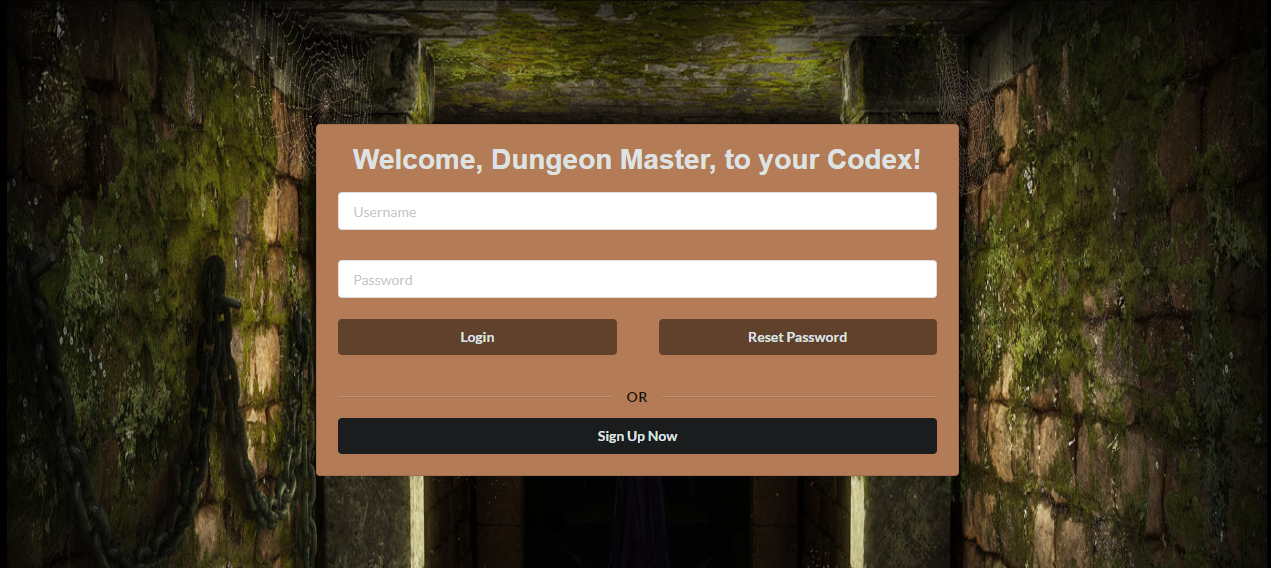
\includegraphics[width=0.8\linewidth]{homepage-developed.png}
			\caption[Screenshot of the \Codex \ web app]{Screenshot taken from the \Codex \ web app homepage which shows the rendered components detailed in Listing \ref{cod:homepage}} \label{fig:homepage}
		\end{figure}
	
		The development of \Codex \ was driven by tests, using the Test Driven Development (TDD) principle, in that each method will produce a testable outcome. Before any development could begin, the developer wrote a test that would ensure no build of the \Codex \ web app would be deployed when the components where unable to be rendered. This was known as a \emph{smoke test} which has been an industry standard test to include in any automated testing environment for over a decade \citep{testing}. Listing \ref{cod:smoke-test} was the source code that was necessary to perform the smoke test on the \Codex \ web app. When a build of the web app was pushed to the master build on GitHub \citep{github}, the code was automatically tested by the web service \emph{CodeShip} \citep{codeship} which would execute the \texttt{App.test.js} file before committing the changes to GitHub. As previously mentioned in Section \ref{sec:agile-solo}, TDD does not prevent every bug from infecting the master version of a project, TDD would prevent the majority of the developer errors increasing the quality of the code produced.
		
		\begin{lstlisting}[caption={\Codex \ web app smoke test}, label={cod:smoke-test}]
		import React from 'react';
		import ReactDOM from 'react-dom';
		import App from './App';
		
		it('renders without crashing', () => {
			const div = document.createElement('div');
			ReactDOM.render(<App />, div);
			ReactDOM.unmountComponentAtNode(div);
		});
		\end{lstlisting}
		
	\section{Outcome of the \Codex \ project} \label{sec:outcomes}
	In this Section we will examine the development of the \Codex \ web app (see Section \ref{sec:dev-obs} and the effectiveness of Agile Solo in managing the development (see Section \ref{sec:agile-solo-effect}). At the end of this section we will have an understanding of the outcomes of the \Codex \ project and will then be able to evaluate those outcomes in Section \ref{sec:evaluation}.
	
		\subsection{Development Observations} \label{sec:dev-obs}
		The \Codex \ web app was developed in ReactJS (see Section \ref{sec:react-js}) using the Software Engineering Methodology (see Section \ref{sec:what-se}) known as Agile Solo (see Sections \ref{sec:agile-solo} and \ref{sec:use-agile-solo}). The effect that Agile Solo had on the development will be discussed in Section \ref{sec:agile-solo-effect}), in this subsection we will discuss the observations the developer recorded during the development stages of the \Codex \ web app. 
		
		The developer had allocated a total of 9 weeks for the development of the \Codex \ web app with an additional 7 weeks for the design of the system. This was found to be insufficient for the a web app such as \Codex \ as the developer found that only the core functionality was able to be achieved within this time frame. The reasons for this were two-fold. The scope of this web app was too great to be tackled within the development time, particularly as the developer was learning ReactJS during the development. Whilst the rate of development increased rapidly as the developer came to understand the nuances of ReactJS (as described in Section \ref{sec:codex-development}), the deadlines of other projects were obtrusive towards the development of \Codex. 
		
		During the implementation the database that supported the app was populated with a small sample of the \WotC \ \dnd \ material. The developer observed that there was no need to transcribe over five hundred pages of statistical data from the \dnd \ core books (Monster Manual, Dungeon Master's Guide and Player's Handbook) and supplementary material (such as Volo's Guide to Monsters \citep{Volo}). The smaller database would allow the development of critical features of \Codex \ to begin earlier than scheduled and be tested with a more manageable dataset. The database would be fully populated at a later date of development. 
		
		Another observation that the developer made during the development of the \Codex \ web app was that the primary function and goal of the development was to provide a platform for the evaluation of Agile Solo. At the end of the scheduled development time, the developer made the conscious and informed decision to prioritise the evaluation of Agile Solo. Development of the web app continued at a slower rate with the change of focus for the project.
					
		\subsection{Effectiveness of Agile Solo} \label{sec:agile-solo-effect}
		[time management]
		
		[task management]
		
		[TDD]
		
		
	\section{Evaluation of \Codex} \label{sec:evaluation}
	boo
	
		\subsection{Feedback on the \Codex \ app} \label{sec:feedback}
		[Chaos report categorisation criteria]
	
		[Testing the web app from a developer point of view]
	
		[Testing the web app from a potential user point of view, limitations from the \WotC \ agreement and gathering feedback]
	
		[Tis a challenged project it is]
		
		\subsection{Development Issues} \label{sec:dev-eval}
		boo
			
		\subsection{Agile Solo Evaluation} \label{sec:agile-solo-eval}
		boo
			
	\section{Conclusions} \label{sec:conclusions}
	The \Codex \ project was to software engineer a progressive web app built in ReactJS, using an agile methodology. The principle challenge of \Codex \ was that, unlike the majority of software engineering project, there was only one developer. Agile methodologies are designed to be used by a group or groups of developers, with designated roles for individuals within the team. As part of the preparation for \Codex, a single developer methodology had to be found, these were \AgileSolo \ and \emph{XP for One}. Agile Solo was selected to be the principle methodology for the development of \Codex. 
	
		\subsection{Agile Solo} \label{sec:agile-solo-conc}
		Agile Solo, as described in Section \ref{sec:agile-solo}, is a methodology that was developed because there was no Agile development methodology designed for solo developer projects. The purpose of a software engineering methodology is to provide a platform to assist with time and task management for a project, in that respect we need to have a certain amount of discipline from the developer when applying a methodology to a project. [It was this discipline that came a critical issue with a solo developer project. When working in a team, each developer is held accountable by the rest of the team. But in solo developer projects no one is holding the developer to account, with the notable exception of a supervisor when present.] However, Agile Solo functioned without flaw when implemented as the original author described. This is evidenced by the project journal, which can be found in the \Codex \ portfolio, where there are numerous entries that prove the following of Agile Solo. The work that was allocated each cycle was achieved and any issues in time spent of that work was down to an incorrect estimation during the allocation process.
		
		In summary, Agile Solo has proven to be a highly effective and accurate methodology for solo developer projects. The methodology proposed in 2011 by Nyst{\"o}m does not need any alterations as far as \Codex \ is concerned.  
		
		\subsection{\Codex} \label{sec:codex-conc}
		\begin{itemize}
			\item The Codex app was a large ambitious project with many complicated features
			\item Developed in a new language to the developer
			\item Developer achieved a working system that provided the core functionality of the app that met the requirements
			\item Many advanced features are easily integrated with more work
			\item Project was not a success as all features were not completed, however it was not a failure as the requirements were satisfied
			\item Therefore the \Codex \ app is a challenged project in accordance with the Standish Group Chaos Report classifications
		\end{itemize}
	
	\clearpage	
	\bibliography{projectbib}
\end{document}
% EOF Document